\documentclass[aspectratio=169,11pt]{beamer}
\usepackage[utf8]{inputenc}
\usepackage[T1]{fontenc}
\usepackage[brazilian]{babel}  
\usepackage{amsmath,amssymb}
\usetheme{Madrid}
\setbeamertemplate{navigation symbols}{}
\newcommand{\todo}[1]{\textcolor{red}{\textbf{[#1]}}}
\title{Treinamento de regressão logística para previsão de \textit{churn}}
\subtitle{Método de Cauchy com busca exata contra Newton puro}
\author{Gabriel Mocellin, Kauan Tomkiel, Luis Veiga, Rogério Ruviaro}
\institute{UFPR --- Programação Não Linear}
\date{}

\begin{document}
\begin{frame}\titlepage
\end{frame}

\begin{frame}{Motivação e objetivo}
\begin{itemize}
    \item Empresas de telecomunicações buscam identificar clientes com maior probabilidade de cancelar seus serviços (\textit{churn}).
    \item A regressão logística permite estimar essas probabilidades a partir das características dos clientes.
    \item O treinamento do modelo consiste em estimar seus parâmetros por meio da \textbf{minimização de uma função objetivo}.
\end{itemize}

\vspace{3mm}
\begin{block}{Objetivo}
Investigar e comparar o método de Cauchy, com busca linear exata, e o método de Newton puro na resolução do problema de otimização associado ao treinamento da regressão logística.
\end{block}
\end{frame}

\begin{frame}{Os dados}
\begin{itemize}
    \item Base pública e fictícia de clientes de telecomunicações:
    \begin{itemize}
        \item $7.043$ observações;
        \item variável resposta binária: cancelamento ou permanência.
    \end{itemize}

    \item Divisão estratificada: $80\%$ para treino ($m=5.634$) e $20\%$ para teste ($1.409$).

    \item Foram selecionadas $9$ variáveis explicativas. Após o pré-processamento, cada observação é representada por $14$ atributos, incluindo o intercepto.

    \item Variáveis numéricas padronizadas pelo Z-score, com parâmetros calculados exclusivamente no conjunto de treino:
\end{itemize}

\[
z_{ij}=\frac{x_{ij}-\mu_j}{\sigma_j}.
\]

\end{frame}

\begin{frame}{Os dados: estrutura do vetor de pesos}
\small
\centering
\renewcommand{\arraystretch}{1.15}
\begin{tabular}{@{}l p{8.2cm} l@{}}
\hline
\textbf{Índice do peso} & \textbf{Atributo correspondente em $X$} & \textbf{Tipo / Natureza} \\ \hline
$w_0$ & Intercepto (coluna unitária) & Constante \\
$w_1$ & \textit{Age} (idade do cliente, 19 a 80 anos) & Numérica (Z-score) \\
$w_2$ & \textit{Tenure in Months} (tempo de vínculo, 1 a 72 meses) & Numérica (Z-score) \\
$w_3$ & \textit{Monthly Charge} (valor da mensalidade) & Numérica (Z-score) \\
$w_4$ & \textit{Number of Referrals} (quantidade de indicações) & Numérica (Z-score) \\
$w_5$ & \textit{Paperless Billing} (fatura digital) & Binária ($\{0,1\}$) \\
$w_6$ & \textit{Married} (estado civil) & Binária ($\{0,1\}$) \\
$w_7,\,w_8$ & \textit{Contract\_One Year}, \textit{Contract\_Two Year} & Binárias (One-Hot) \\
$w_9,\,w_{10},\,w_{11}$ & \textit{Internet Type\_DSL}, \textit{Fiber Optic}, \textit{None} & Binárias (One-Hot) \\
$w_{12},\,w_{13}$ & \textit{Payment Method\_Credit Card}, \textit{Mailed Check} & Binárias (One-Hot) \\ \hline
\end{tabular}

\vspace{3mm}
\raggedright\footnotesize Estrutura do vetor de pesos $w\in\mathbb{R}^{14}$ e correspondência com as colunas da matriz $X$.
\end{frame}

\begin{frame}{Regressão logística}
A regressão logística modela o logaritmo da razão de chances como uma função linear dos atributos:

\[
\ln\left(
\frac{P(y_i=1\mid x_i;w)}
{1-P(y_i=1\mid x_i;w)}
\right)=x_i^\top w.
\]

Isolando a probabilidade de cancelamento, obtemos a função sigmoide:

\[
\hat p_i(w)=\sigma(x_i^\top w),
\qquad
\sigma(z)=\frac{1}{1+e^{-z}},
\]

\vspace{2mm}
em que a saída do modelo é uma probabilidade estimada de cancelamento.
\end{frame}

\begin{frame}{Treinar é minimizar}
A estimação dos parâmetros por máxima verossimilhança equivale a minimizar a entropia cruzada binária média:

\[
f(w)=\frac{1}{m}\sum_{i=1}^{m}
\left[
\ln(1+e^{x_i^\top w})-y_i x_i^\top w
\right].
\]

\vspace{2mm}
\[
\boxed{
\min_{w\in\mathbb{R}^{14}} f(w)
}
\]

\begin{itemize}
    \item Problema de otimização não linear e irrestrita;
    \item $14$ variáveis de decisão;
    \item Sem solução em forma fechada: os parâmetros são obtidos numericamente.
\end{itemize}
\end{frame}

\begin{frame}{Gradiente e Hessiana}
Definindo
\[
D(w)=\operatorname{diag}\big(\hat p_i(w)(1-\hat p_i(w))\big),
\qquad 0<d_{ii}\leq \frac14,
\]
obtemos:

\[
\nabla f(w)=\frac{1}{m}X^\top(\hat p(w)-y),
\]

\[
\nabla^2 f(w)=\frac{1}{m}X^\top D(w)X.
\]

\vspace{3mm}
\begin{itemize}
    \item \textbf{Gradiente:} indica a direção de maior crescimento da função.
    \item \textbf{Hessiana:} descreve a curvatura local e será utilizada para determinar a direção de Newton.
\end{itemize}
\end{frame}

\begin{frame}{Teorema 1: propriedades da função objetivo}
Sob as hipóteses:

\begin{itemize}
    \item \textbf{(H1)} $\operatorname{posto}(X)=n$;
    \item \textbf{(H2)} não existe direção não nula que separe completamente ou quase completamente as classes;
\end{itemize}

temos:

\begin{itemize}
    \item $f\in C^\infty$ e $\nabla^2 f(w)\succ0$ para todo $w$;
    \item existe um único minimizador global $w^*$, com $\nabla f(w^*)=0$;
    \item o gradiente é Lipschitz contínuo, com constante
\end{itemize}

\[
L=\frac{\lambda_{\max}(X^\top X)}{4m}.
\]
\end{frame}

\begin{frame}{Teorema 1: ideia da demonstração}
\textbf{1. Convexidade e convexidade estrita}

\[
v^\top\nabla^2 f(w)v
=
\frac{1}{m}\sum_{i=1}^{m}
d_{ii}(x_i^\top v)^2\geq 0.
\]

Sob H1, a igualdade só ocorre para $v=0$.

\vspace{2mm}
\textbf{2. Gradiente Lipschitz}

Como $d_{ii}\leq \frac14$, obtemos

\[
\nabla^2 f(w)\preceq
\frac{1}{4m}X^\top X\preceq LI.
\]

\vspace{2mm}
\textbf{3. Existência do minimizador}

Sob H2, $f$ é coerciva. Pela continuidade e pelo Teorema de Weierstrass, existe um minimizador global, único pela convexidade estrita.
\end{frame}

\begin{frame}{Teorema 2: propriedades no conjunto de subnível}
Sob H1 e H2, para um ponto inicial $w^0$, considere

\[
S=\{w\in\mathbb{R}^n:f(w)\leq f(w^0)\}.
\]

Então:

\begin{itemize}
    \item $S$ é não vazio, compacto e convexo;
    \item existem constantes $\mu>0$ e $L>0$ tais que, em $S$,
\end{itemize}

\[
\boxed{
\mu I\preceq\nabla^2 f(w)\preceq LI
}
\]

\vspace{2mm}
\textbf{Consequência:} $f$ é fortemente convexa e possui gradiente Lipschitz contínuo nesse conjunto.
\end{frame}

\begin{frame}{Método de Cauchy (Gradiente)}

\textbf{Direção de busca:}
\[
d^k=-\nabla f(w^k).
\]

\textbf{Tamanho do passo (busca linear exata):}
\[
t_k=\arg\min_{t\geq0}f(w^k+td^k).
\]

\textbf{Atualização:}
\[
\boxed{w^{k+1}=w^k+t_kd^k}
\]

\begin{itemize}
    \item O passo é determinado numericamente pelo método da seção áurea;
    \item A busca exata garante que $f(w^{k+1})\leq f(w^k)$.
\end{itemize}

\end{frame}

\begin{frame}{Cauchy: convergência}
Sob as condições do Teorema 2, o método de Cauchy com busca linear exata apresenta convergência global e linear:

\[
f(w^{k+1})-f(w^*)
\leq
\left(1-\frac{\mu}{L}\right)
\left[f(w^k)-f(w^*)\right].
\]

\vspace{3mm}
\begin{itemize}
    \item A taxa depende da razão de condicionamento $L/\mu$;
    \item Problemas mal condicionados podem apresentar convergência lenta;
    \item As curvas de nível alongadas podem provocar trajetórias em zigue-zague.
\end{itemize}
\end{frame}

\begin{frame}{Método de Newton puro}
\[ \nabla^2 f(w^k)\, d^k = -\nabla f(w^k), \qquad w^{k+1} = w^k + d^k \quad (t_k = 1). \]
\begin{itemize}
\item Pelo Teorema 1, o sistema tem solução única e $d^k$ é sempre direção de descida.
\item Perto de $w^*$: convergência \textbf{quadrática}.
\item Longe de $w^*$: o passo unitário pode não decrescer $f$. Com a sigmoide saturada, $d_{ii} \approx 0$ e a Hessiana fica quase singular, produzindo passos enormes.
\end{itemize}
\end{frame}

\begin{frame}{Implementação e pipeline do código}
\centering
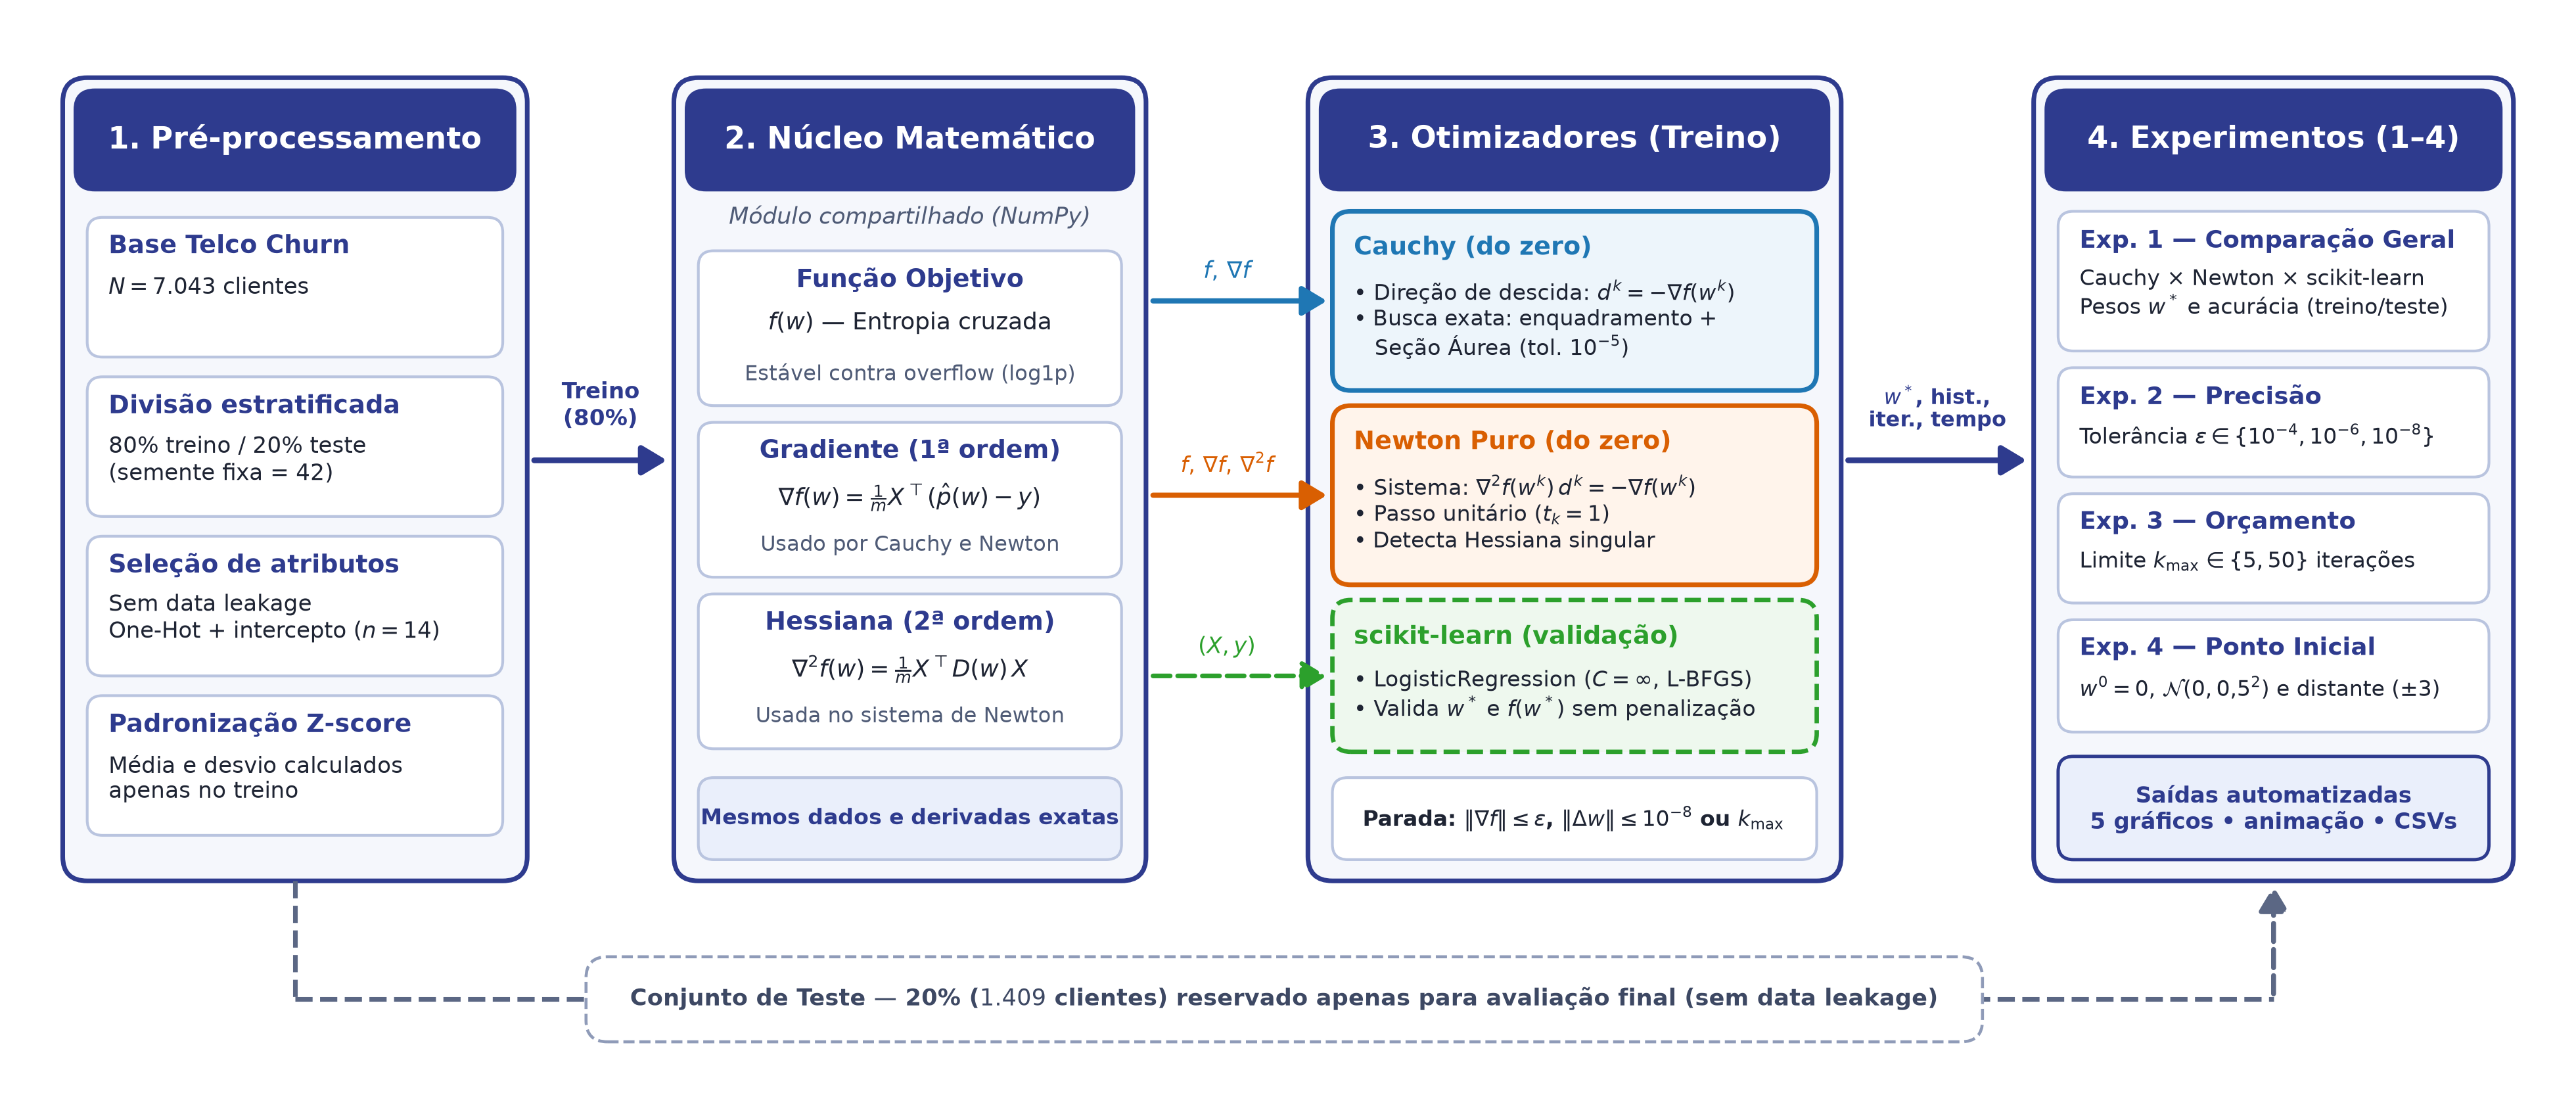
\includegraphics[width=\textwidth,height=0.65\textheight,keepaspectratio]{../imgs/experimentos/00_arquitetura_pipeline.png}
\vspace{1.5mm}

\footnotesize\raggedright
\begin{itemize}
\setlength{\itemsep}{2pt}
\item \textbf{Stack e modularidade:} \texttt{Python 3.13} (\texttt{NumPy}, \texttt{Pandas}, \texttt{scikit-learn}, \texttt{Matplotlib}), orquestrado em \texttt{main.py}.
\item \textbf{Núcleo compartilhado:} $f(w)$ estável (\texttt{log1p}), $\nabla f$ e $\nabla^2 f$ exatos; Cauchy e Newton implementados do zero.
\item \textbf{Reprodutibilidade:} semente fixa (\texttt{42}), teste isolado (sem \textit{data leakage}) e geração automática de figuras e CSVs.
\end{itemize}
\end{frame}

\begin{frame}{Experimento 1: configuração e comparação geral}
\begin{itemize}
\item Padrão: $w^0 = 0$, $\|\nabla f(w^k)\| \le 10^{-6}$, $\|w^{k+1}-w^k\| \le 10^{-8}$, $k_{\max} = 1000$ e seção áurea com tolerância $10^{-5}$.
\item Validação contra \texttt{scikit-learn} (\texttt{C=np.inf}, \texttt{tol=1e-6}, solver L-BFGS).
\end{itemize}
\vspace{2mm}
\centering
\small
\begin{tabular}{lccc}
\toprule
\textbf{Métrica} & \textbf{Cauchy} & \textbf{Newton puro} & \textbf{Scikit-Learn} \\
\midrule
Iterações & $338$ & $6$ & $35$ \\
Tempo (s) & $1{,}634$ & $0{,}005$ & $0{,}023$ \\
$\|\nabla f(w^*)\|$ (treino) & $9{,}60 \times 10^{-7}$ & $1{,}32 \times 10^{-7}$ & $1{,}54 \times 10^{-6}$ \\
$f(w^*)$ treino / teste & $0{,}367535$ / $0{,}365378$ & $0{,}367535$ / $0{,}365378$ & $0{,}367535$ / $0{,}365378$ \\
Acurácia treino / teste & $83{,}00\%$ / $82{,}54\%$ & $83{,}00\%$ / $82{,}54\%$ & $83{,}00\%$ / $82{,}54\%$ \\
\bottomrule
\end{tabular}
\end{frame}

\begin{frame}{Experimento 1: convergência (Cauchy $\times$ Newton)}
\centering
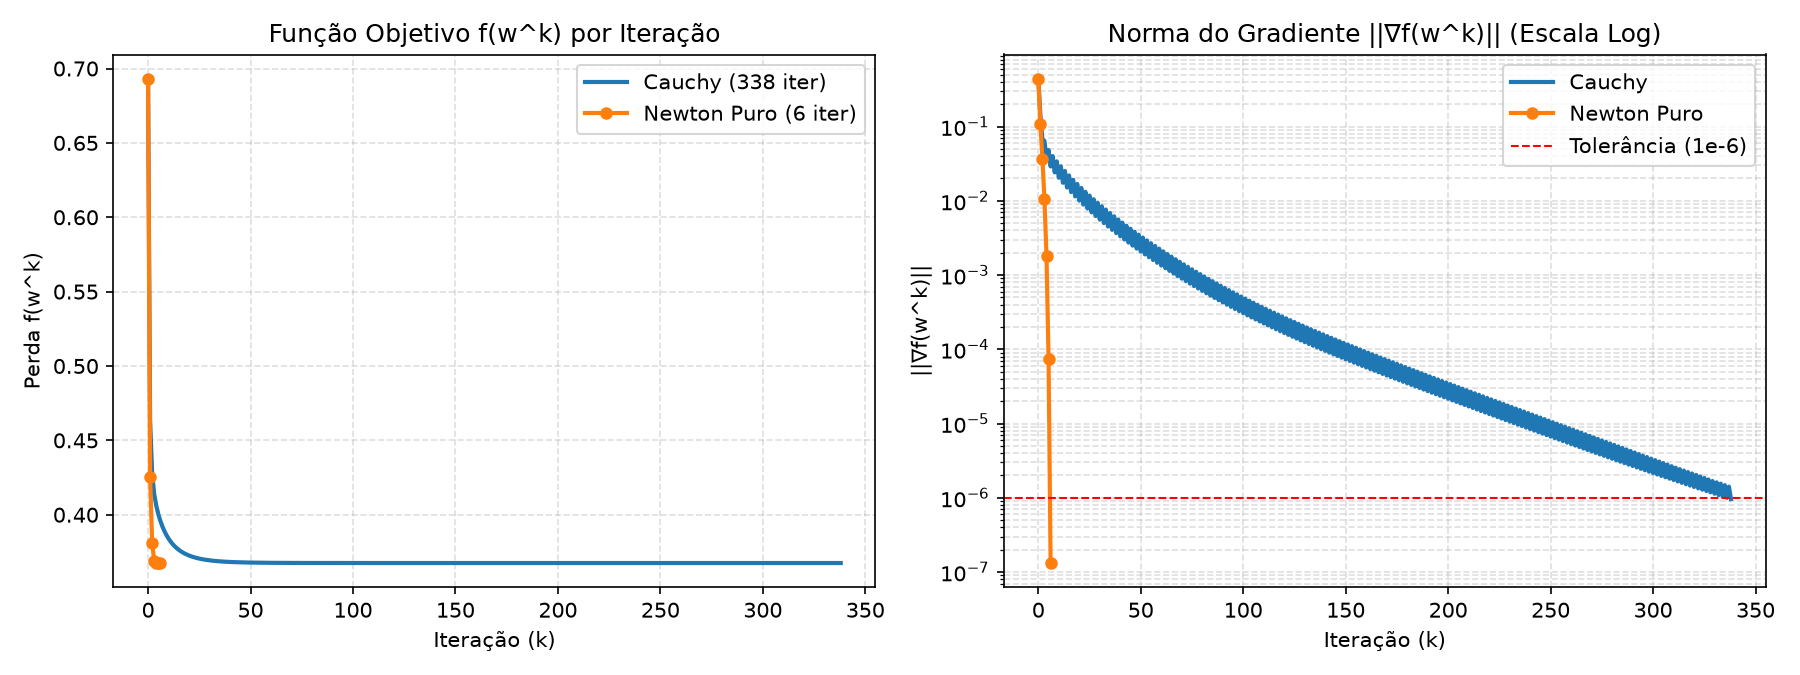
\includegraphics[width=\textwidth,height=0.72\textheight,keepaspectratio]{../imgs/experimentos/01_exp1_convergencia.png}
\vspace{1mm}

\small\raggedright
Convergência \textbf{linear} com zigue-zague no Cauchy ($338$ iter) contra queda \textbf{quadrática} no Newton puro ($6$ iter).
\end{frame}

\begin{frame}{Experimento 1: pesos ótimos e desempenho (Treino $\times$ Teste)}
\centering
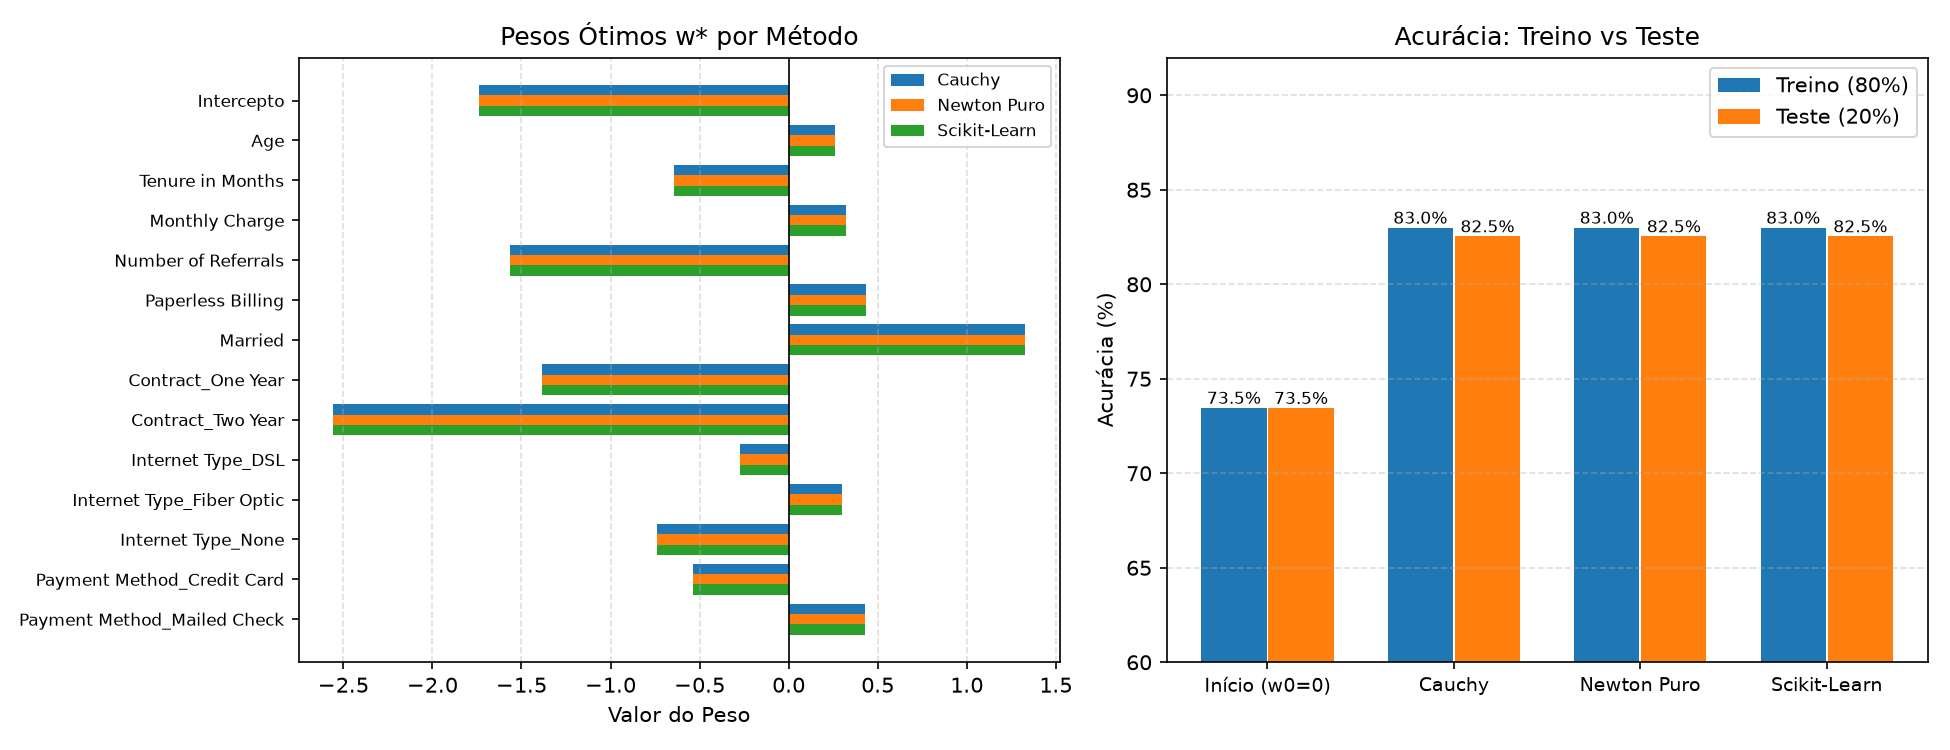
\includegraphics[width=\textwidth,height=0.72\textheight,keepaspectratio]{../imgs/experimentos/02_exp1_pesos_e_desempenho.png}
\vspace{1mm}

\small\raggedright
Os três métodos convergem aos mesmos pesos $w^*$; acurácia sobe de $73{,}5\%$ ($w^0 = 0$) para $83{,}0\%$ no treino e $82{,}5\%$ no teste.
\end{frame}

\begin{frame}{Experimento 2: influência da precisão ($\varepsilon \in \{10^{-4}, 10^{-6}, 10^{-8}\}$)}
\centering
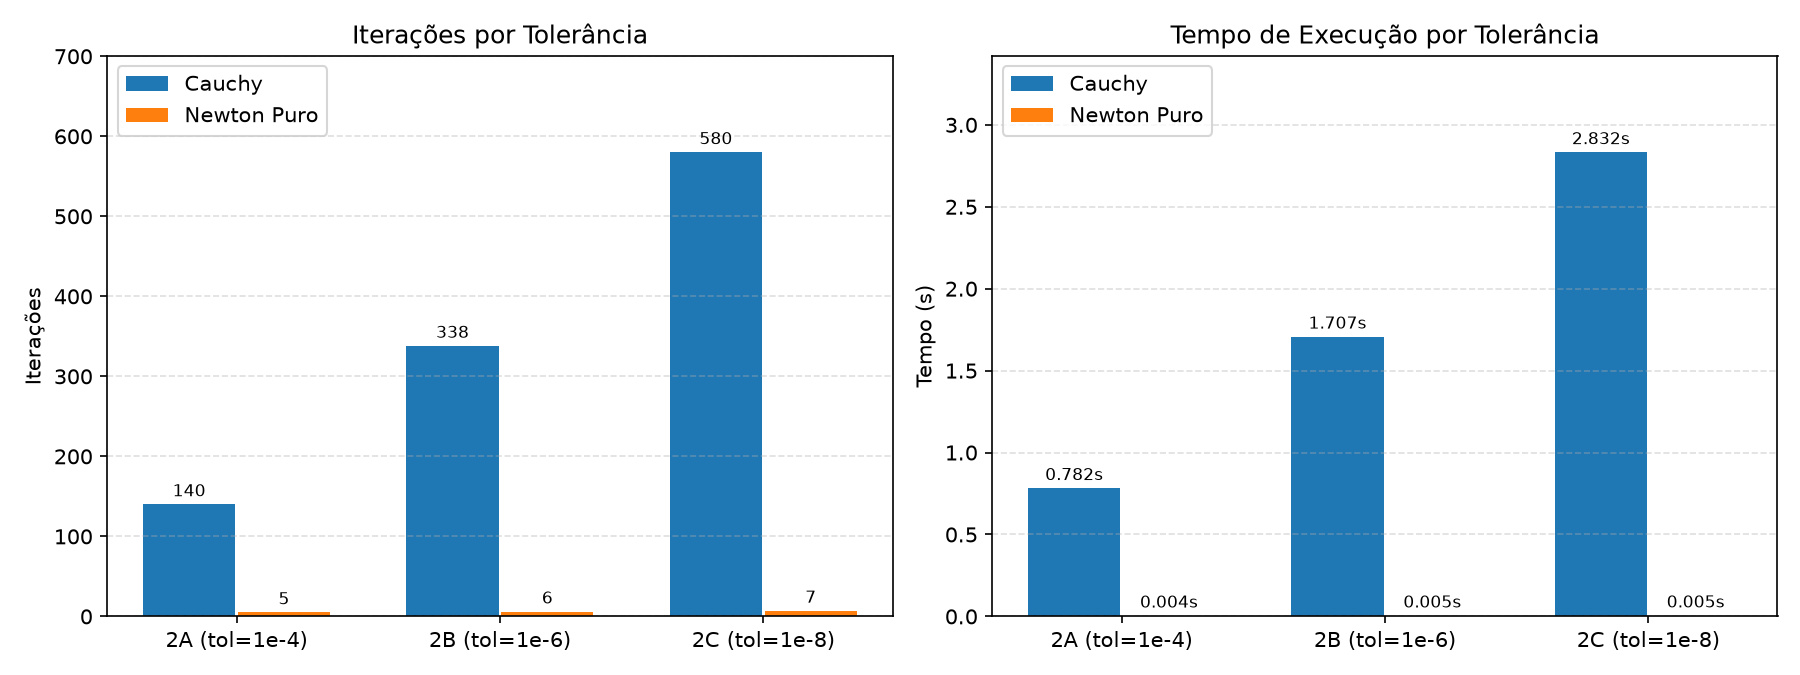
\includegraphics[width=\textwidth,height=0.70\textheight,keepaspectratio]{../imgs/experimentos/03_exp2_precisao.png}
\vspace{1mm}

\small\raggedright
De $10^{-4}$ para $10^{-8}$, Cauchy salta de $140$ para $580$ iterações ($0{,}782$\,s $\to 2{,}832$\,s); Newton vai de $5$ para $7$ iterações ($\|\nabla f\| = 4{,}24 \times 10^{-13}$).
\end{frame}

\begin{frame}{Experimento 3: limite máximo de iterações ($k_{\max} \in \{5, 50\}$)}
\centering
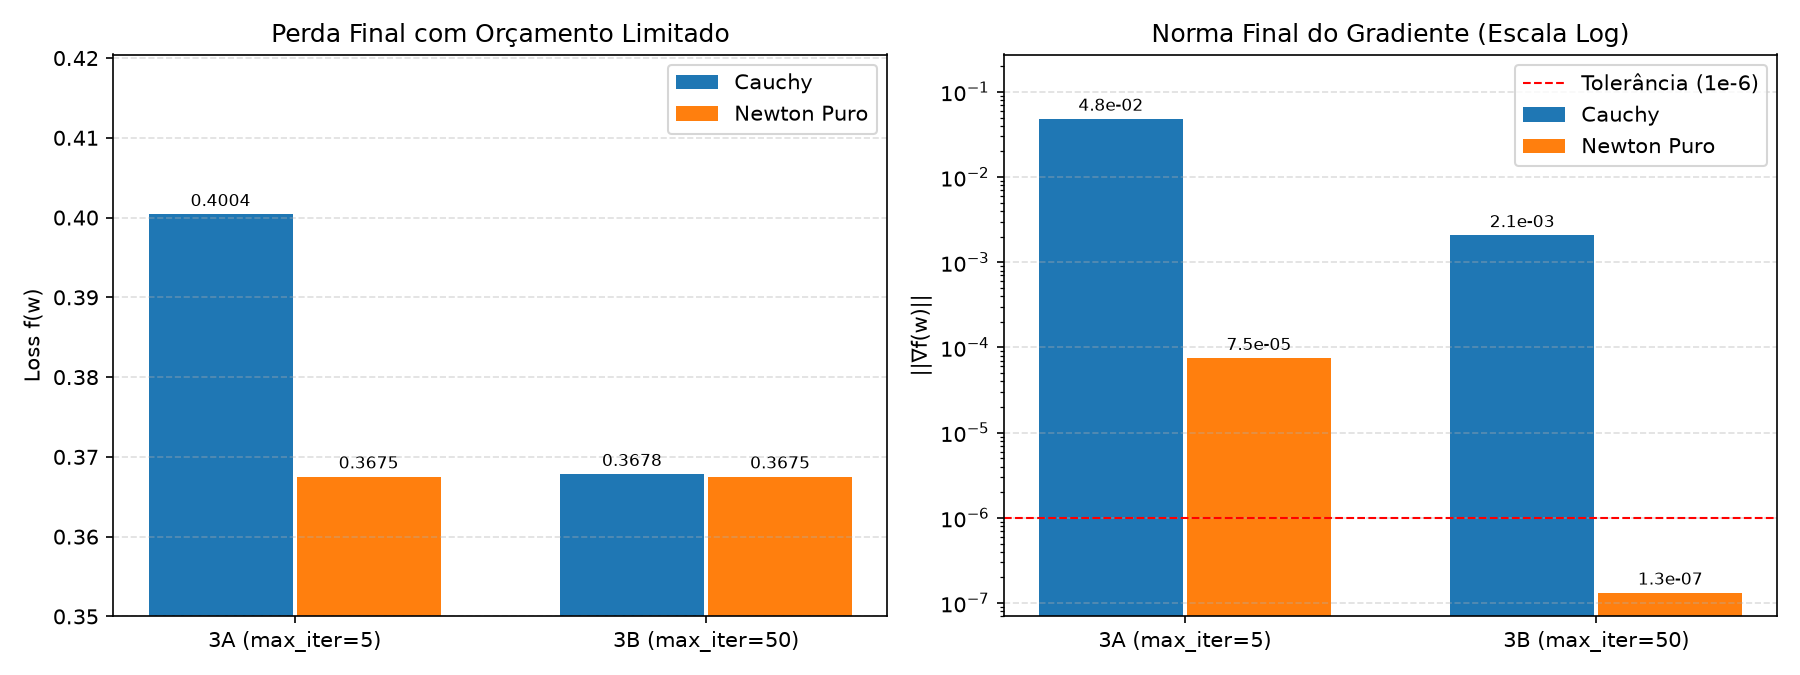
\includegraphics[width=\textwidth,height=0.70\textheight,keepaspectratio]{../imgs/experimentos/04_exp3_limite_iteracoes.png}
\vspace{1mm}

\small\raggedright
Com $k_{\max} = 5$, Newton já alcança $f = 0{,}3675$ ($\|\nabla f\| = 7{,}5 \times 10^{-5}$); com $k_{\max} = 50$, Newton converge na iteração $6$, enquanto Cauchy permanece em $\|\nabla f\| = 2{,}1 \times 10^{-3}$.
\end{frame}

\begin{frame}{Experimento 4: sensibilidade ao ponto inicial $w^0$}
\centering
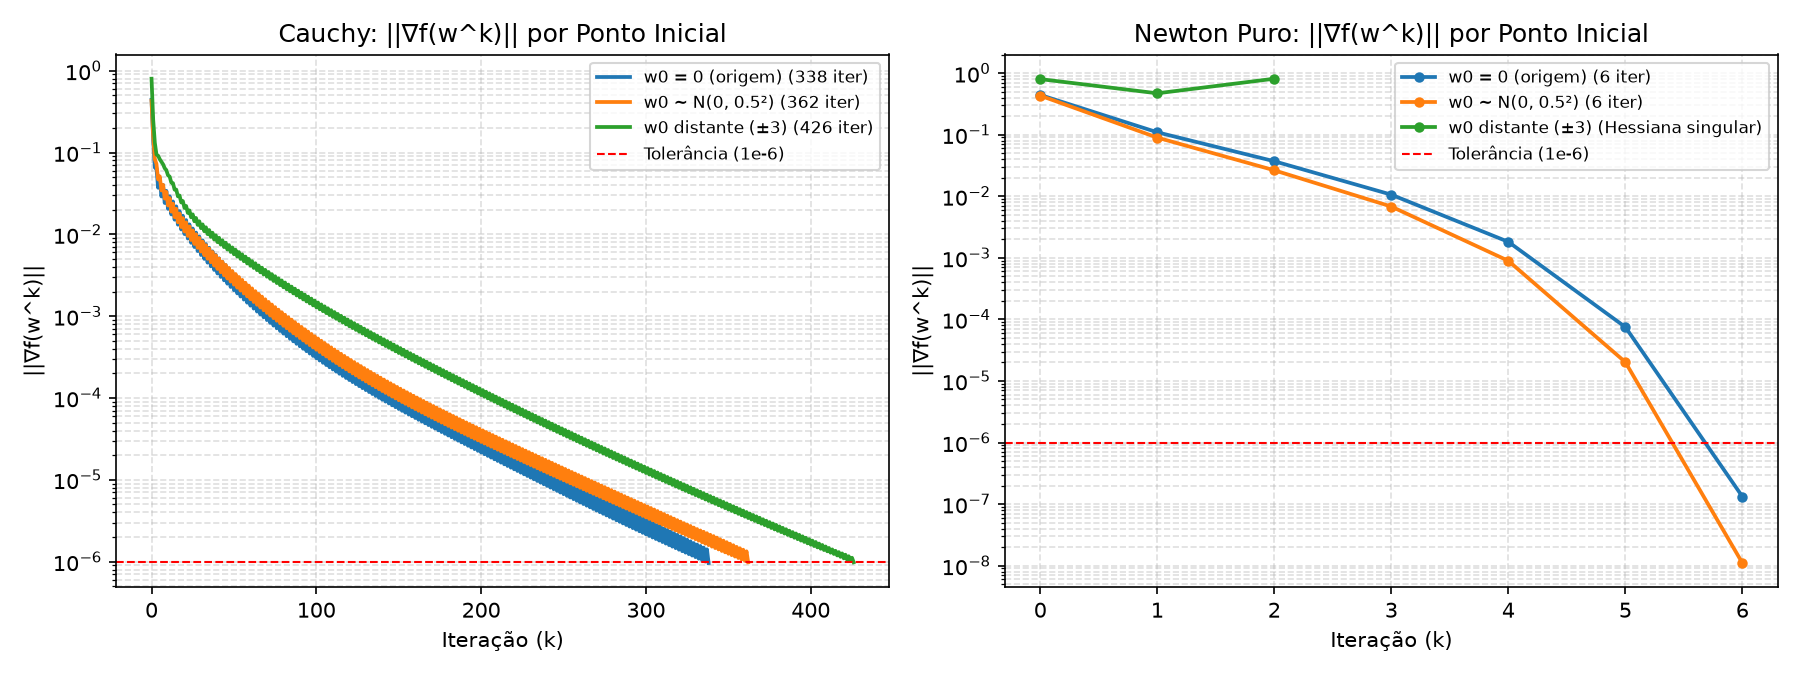
\includegraphics[width=\textwidth,height=0.70\textheight,keepaspectratio]{../imgs/experimentos/05_exp4_pontos_iniciais.png}
\vspace{1mm}

\small\raggedright
Cauchy converge em todos os cenários ($338$, $362$ e $426$ iter). Newton converge em $6$ iter perto da origem, mas falha na iteração $2$ (\textit{Hessiana singular}) em $w^0 = \pm 3$.
\end{frame}

\begin{frame}{Conclusões}
\begin{itemize}
\item Treinar a regressão logística é um problema irrestrito, suave e convexo; sob H1 e H2 há minimizador global único.
\item Os experimentos confirmaram a teoria: convergência linear no Cauchy ($338$ iter) e quadrática local no Newton puro ($6$ iter, $0{,}005$\,s).
\item Maior precisão penaliza fortemente o Cauchy ($580$ iter para $10^{-8}$), mas quase não altera o Newton ($7$ iter).
\item Longe da solução ($w^0 = \pm 3$), apenas o Cauchy convergiu; o Newton puro falhou por saturação da sigmoide e Hessiana singular.
\item Ambos reproduziram os pesos e a acurácia do \texttt{scikit-learn} ($83{,}00\%$ no treino e $82{,}54\%$ no teste).
\end{itemize}
\end{frame}


\end{document}